\documentclass{article}

\usepackage[final]{neurips_2019}
\usepackage[utf8]{inputenc} % allow utf-8 input
\usepackage[T1]{fontenc}    % use 8-bit T1 fonts
\usepackage{hyperref}       % hyperlinks
\usepackage{url}            % simple URL typesetting
\usepackage{booktabs}       % professional-quality tables
\usepackage{amsfonts}       % blackboard math symbols
\usepackage{nicefrac}       % compact symbols for 1/2, etc.
\usepackage{microtype}      % microtypography
\usepackage{graphicx}
\graphicspath{ {./images/} }


\title{Music Classification Using Convolutional Neural Networks}

\author{%
Abel Putovici\And
Zsombor Molnár
}

\begin{document}

    \maketitle

    \begin{abstract}
        The abstract paragraph should be indented \nicefrac{1}{2}~inch (3~picas) on
        both the left- and right-hand margins. Use 10~point type, with a vertical
        spacing (leading) of 11~points. The word \textbf{Abstract} must be centered,
        bold, and in point size 12. Two line spaces precede the abstract. The abstract
        must be limited to one paragraph.
    \end{abstract}

    \section{Introduction}

    Music is and has always been one of the most popular forms of art and
    entertainment. The number of people who use streaming services to consume music
    has grown to a magnitude of millions in this decade. These services make use of
    complicated and complex recommender systems to help grow the number of
    daily active users and to improve their experience of the service. These recommender
    systems rely on extremely large labeled datasets in order to work properly, and
    labeling these datasets manually is a very resource-heavy endeavour.

    \subsection{Our Goal}

    \paragraph{Music Genres in General}

    One possible way of labeling songs is doing it by genre though this introduces
    other difficulties, since these are ment to indicate the artistic nature of music, an
    aspect which tends to be highly subjective and controversial. Music genres do not have a
    proper, formal definition and often overlap as well, making music classification by
    genre a more difficult task to do right.

    \paragraph{Our Primary Goal}

    Our primary goal was do deliver a solution which can effectively recognize some of the
    most popular and generic music genres and assign these as labels to songs of music.

    \section{Our Approach}

    There are many existing solutions and research papers regarding the subject and these
    show absolutely usable methods and results, though each of them tend to have a major
    drawback: every solution aims to work in \emph{centralized environments} due to their
    computational requirements. We decided that our approach had to be able to work on
    edge devices such as smart phones or other, more constrained environments, even on
    cost of precision. This decision implied a rather small model size and great model
    simplicity, this is why we chose to try a simple convolutional neural network.

	\section{The dataset}

	We wanted to have a great vatiety of song samples in large quantity.
	The first dataset we took into account is the \textit{Million Song Dataset} \cite{million}.
	The sheer number of samples was quite promissing, but it turned out to be overwhelming.
	Not to mention the fact that it contained numerous pieces of information that we did not need, like the authors,
	the release year and other different identifiers for database use. 
	It needed a lot of time just to extract the necessary information we need, which would make the extension 
	of the used dataset unnecessarily time consuming. 


	Our second option was the GTZAN \cite{gtzan_art} dataset used in the \textit{Musical genre classification of audio signals} \cite{gtzan}.
	It suited our needs and it covered samples from 10 clearly distinct music genres, 100 tracks each.
	As for the length of the songs, the dataset contained 30 second long samples from different parts of the songs.
	An analysis done by Bob L. Strum \cite{gtzan_anal} describes more precisely the capacity of this dataset.

    \section{The Model}

    \subsection{Trial and Error}

    We went through numerous iterations and tried various convolutional neural
    network architectures during development. At first we tried to use convolutional
    windows that would overlap the whole frequency domain and move only in the time domain,
    since although spectrograms can be regarded as arbitrary two dimensional data, the two
    axises have different meanings. This path led nowhere, the model was not able to
    overfit on a small subset of the dataset. We decided to use simple, rectangular convolutional
    windows, which could be called standard by now. This approach was indeed able to overfit, meaning
    it was worth to try learning on the whole dataset. Validation error would cease to decrease
    after the first few epochs. This would be followed by decreasing the input size of the model
    by splitting the samples of 30 seconds length into 4 smaller fragments.

    \subsection{The Final Model Architecture}

    The final model consists of the following layers:

    \begin{itemize}
        \item a convolutional layer with a depth of 32 and a window shape of (2, 6)
        \item another convolutional layer with a depth of 32 and a window shape of (2, 6)
        \item a convolutional layer with a depth of 64 and a window shape identical to the previous ones
        \item a fully connected layer of 512 neurons
    \end{itemize}

    Each convolutional layer was followed by a batch normalization
    layer and a max-pooling layer. L1 and L2 regularizers were adopted to the fully connected layer.
    The model has an output layer of 10 neurons with \emph{softmax} as activation function.

    \subsection{Hyperparameters}
    \paragraph{Activation functions}
    At first we tried using \emph{ReLU} activations between each layer. This lead to many issues,
    since in the context of Mel spectrograms negative numbers have significance. Perceiving this,
    we decided to use \emph{Hyperbolic Tangent} as activation function.

    \paragraph{Loss Function}
    The loss function used is \emph{Sparse Categorical Crossentropy} since the labels are not one-hot encoded.

    \paragraph{Optimizer}
    The optimizer algorithm used during training was Stochastic Gradient Descent with a learning rate of 0.01.
    At first we've tried with \emph{Adam} but it did not perform quite as expected. The next choice
    was \emph{Adadelta} which showed promising results, but it did not appear to stable due to the
    fluctuation we have observed on both the graphs of training and validation accuracy.

    \paragraph{Number of Epoch and Data Split}
    The model was trained for 100 epochs with a batch size of 5. 80 percent of the data was used
    for training, 10 percent was used for validation and the last 10 percent was used for testing.

    \paragraph{Vanishing Gradient}

    During the training process we've noticed that after a certain number of epochs
    the validation accuracy would cease to converge. This was due to the Vanishing
    Gradient problem, which led to the choice of using \emph{Linear} activation between the
    convolutional layers, leaving \emph{Hyperbolic Tangent} only between the output and
    the fully connected layer.

    \section{Results}

    \subsection{Training and Validation}

    The model is still overfitting with the validation accuracy being stuck at \~60\% and the training accuracy soaring.

    \begin{center}
        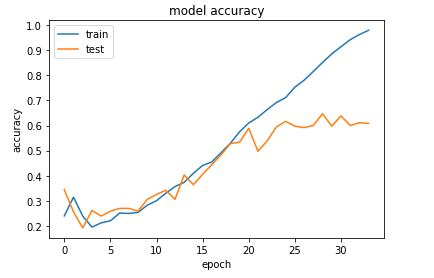
\includegraphics[scale=0.5]{acc}
        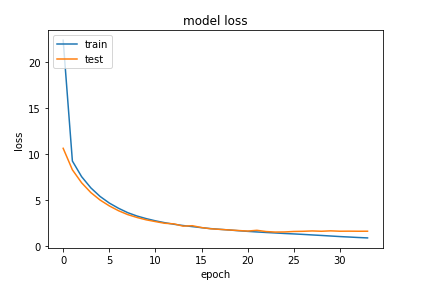
\includegraphics[scale=0.5]{loss}
    \end{center}

    \subsection{Testing Accuracy}

    The final testing accuracy of the model is \textbf{0.61\%}. Below are the Classication Matrix and the final
    Classification Report.

    \begin{table}[h]
        \caption{Confusion Matrix}
        \centering
        \begin{tabular}{l | llllllllll}
            Genre & Metal & Classical & Reggae & Jazz & Country & Rock & Hiphop & Disco & Pop & Blues \\
            \midrule
            Metal & 44 & 0 & 0 & 0 & 0 & 0 & 0 & 0 & 0 & 0 \\
            Classical & 0 & 28 & 0 & 0 & 1 & 1 & 0 & 0 & 0 & 0 \\
            Reggae & 1 & 1 & 18 & 0 & 1 & 2 & 5 & 3 & 8 & 5 \\
            Jazz & 1 & 11 & 0 & 28 & 1 & 1 & 0 & 0 & 1 & 2 \\
            Country & 0 & 2 & 0 & 3 & 20 & 1 & 0 & 0 & 0 & 4 \\
            Rock & 12 & 0 & 0 & 2 & 5 & 16 & 4 & 2 & 1 & 4 \\
            Hiphop & 7 & 0 & 1 & 0 & 0 & 0 & 28 & 0 & 1 & 2 \\
            Disco & 4 & 1 & 4 & 0 & 1 & 9 & 7 & 8 & 7 & 2 \\
            Pop & 0 & 3 & 1 & 0 & 3 & 2 & 2 & 0 & 35 & 2 \\
            Blues & 1 & 1 & 0 & 5 & 2 & 0 & 0 & 1 & 0 & 20 \\
            \bottomrule
        \end{tabular}
    \end{table}

    \begin{table}[h]
        \caption{Classification Report}
        \centering
        \begin{tabular}{l | l l l l}
            Genre & Precision & Recall & F1-Score & Support (number of samples) \\
            \midrule
            metal & 1.00 & 0.63 & 0.77 & 70 \\
            classical & 0.93 & 0.60 & 0.73 & 47 \\
            reggae & 0.41 & 0.75 & 0.53 & 24 \\
            jazz & 0.63 & 0.74 & 0.68 & 39 \\
            country & 0.67 & 0.59 & 0.62 & 34 \\
            rock & 0.35 & 0.50 & 0.41 & 32 \\
            hiphop & 0.72 & 0.61 & 0.66 & 46 \\
            disco & 0.19 & 0.57 & 0.28 & 14 \\
            pop & 0.73 & 0.66 & 0.69 & 53 \\
            blues & 0.67 & 0.49 & 0.56 & 41 \\
            \bottomrule
        \end{tabular}
    \end{table}

    \begin{table}[h]
        \caption{Classification Report Averages}
        \centering
        \begin{tabular}{l | l l l l}
            Type & Precision & Recall & F1-Score & Support (number of samples) \\
            \midrule
            Macro Average & 0.63 & 0.61 & 0.59 & 400 \\
            Weighted Average & 0.71 & 0.61 & 0.64 & 400 \\
            \bottomrule
        \end{tabular}
    \end{table}

    \section{Future Improvements}

    There are many ways the solution could be improved. Our plans include

    \begin{itemize}
        \item augmenting the dataset by time-stretching (and squeezing) and splitting the 30 second
        samples using slightly overlapping windows
        \item experimenting with different network architectures
        \item applying \emph{Hyperparameter Optimization}
        \item maybe searching for network architectures using experimental solutions like \emph{AutoML}
    \end{itemize}


    \section*{References}

    References follow the acknowledgments. Use unnumbered first-level heading for
    the references. Any choice of citation style is acceptable as long as you are
    consistent. It is permissible to reduce the font size to \verb+small+ (9 point)
    when listing the references. {\bf Remember that you can use more than eight
    pages as long as the additional pages contain \emph{only} cited references.}
    \medskip

    \small

    [1] Alexander, J.A.\ \& Mozer, M.C.\ (1995) Template-based algorithms for
    connectionist rule extraction. In G.\ Tesauro, D.S.\ Touretzky and T.K.\ Leen
    (eds.), {\it Advances in Neural Information Processing Systems 7},
    pp.\ 609--616. Cambridge, MA: MIT Press.

    [2] Bower, J.M.\ \& Beeman, D.\ (1995) {\it The Book of GENESIS: Exploring
    Realistic Neural Models with the GEneral NEural SImulation System.}  New York:
    TELOS/Springer--Verlag.

    [3] Hasselmo, M.E., Schnell, E.\ \& Barkai, E.\ (1995) Dynamics of learning and
    recall at excitatory recurrent synapses and cholinergic modulation in rat
    hippocampal region CA3. {\it Journal of Neuroscience} {\bf 15}(7):5249-5262.

\end{document}
